% Options for packages loaded elsewhere
\PassOptionsToPackage{unicode}{hyperref}
\PassOptionsToPackage{hyphens}{url}
%
\documentclass[
  11pt,
  letterpaper,
  DIV=11,
  numbers=noendperiod,
  twoside]{scrartcl}

\usepackage{amsmath,amssymb}
\usepackage{setspace}
\usepackage{iftex}
\ifPDFTeX
  \usepackage[T1]{fontenc}
  \usepackage[utf8]{inputenc}
  \usepackage{textcomp} % provide euro and other symbols
\else % if luatex or xetex
  \usepackage{unicode-math}
  \defaultfontfeatures{Scale=MatchLowercase}
  \defaultfontfeatures[\rmfamily]{Ligatures=TeX,Scale=1}
\fi
\usepackage{lmodern}
\ifPDFTeX\else  
    % xetex/luatex font selection
    \setmainfont[ItalicFont=EB Garamond Italic,BoldFont=EB Garamond
Bold]{EB Garamond Math}
    \setsansfont[]{EB Garamond}
  \setmathfont[]{Garamond-Math}
\fi
% Use upquote if available, for straight quotes in verbatim environments
\IfFileExists{upquote.sty}{\usepackage{upquote}}{}
\IfFileExists{microtype.sty}{% use microtype if available
  \usepackage[]{microtype}
  \UseMicrotypeSet[protrusion]{basicmath} % disable protrusion for tt fonts
}{}
\usepackage{xcolor}
\usepackage[left=1.1in, right=1in, top=0.8in, bottom=0.8in,
paperheight=9.5in, paperwidth=7in, includemp=TRUE, marginparwidth=0in,
marginparsep=0in]{geometry}
\setlength{\emergencystretch}{3em} % prevent overfull lines
\setcounter{secnumdepth}{3}
% Make \paragraph and \subparagraph free-standing
\makeatletter
\ifx\paragraph\undefined\else
  \let\oldparagraph\paragraph
  \renewcommand{\paragraph}{
    \@ifstar
      \xxxParagraphStar
      \xxxParagraphNoStar
  }
  \newcommand{\xxxParagraphStar}[1]{\oldparagraph*{#1}\mbox{}}
  \newcommand{\xxxParagraphNoStar}[1]{\oldparagraph{#1}\mbox{}}
\fi
\ifx\subparagraph\undefined\else
  \let\oldsubparagraph\subparagraph
  \renewcommand{\subparagraph}{
    \@ifstar
      \xxxSubParagraphStar
      \xxxSubParagraphNoStar
  }
  \newcommand{\xxxSubParagraphStar}[1]{\oldsubparagraph*{#1}\mbox{}}
  \newcommand{\xxxSubParagraphNoStar}[1]{\oldsubparagraph{#1}\mbox{}}
\fi
\makeatother


\providecommand{\tightlist}{%
  \setlength{\itemsep}{0pt}\setlength{\parskip}{0pt}}\usepackage{longtable,booktabs,array}
\usepackage{calc} % for calculating minipage widths
% Correct order of tables after \paragraph or \subparagraph
\usepackage{etoolbox}
\makeatletter
\patchcmd\longtable{\par}{\if@noskipsec\mbox{}\fi\par}{}{}
\makeatother
% Allow footnotes in longtable head/foot
\IfFileExists{footnotehyper.sty}{\usepackage{footnotehyper}}{\usepackage{footnote}}
\makesavenoteenv{longtable}
\usepackage{graphicx}
\makeatletter
\newsavebox\pandoc@box
\newcommand*\pandocbounded[1]{% scales image to fit in text height/width
  \sbox\pandoc@box{#1}%
  \Gscale@div\@tempa{\textheight}{\dimexpr\ht\pandoc@box+\dp\pandoc@box\relax}%
  \Gscale@div\@tempb{\linewidth}{\wd\pandoc@box}%
  \ifdim\@tempb\p@<\@tempa\p@\let\@tempa\@tempb\fi% select the smaller of both
  \ifdim\@tempa\p@<\p@\scalebox{\@tempa}{\usebox\pandoc@box}%
  \else\usebox{\pandoc@box}%
  \fi%
}
% Set default figure placement to htbp
\def\fps@figure{htbp}
\makeatother
% definitions for citeproc citations
\NewDocumentCommand\citeproctext{}{}
\NewDocumentCommand\citeproc{mm}{%
  \begingroup\def\citeproctext{#2}\cite{#1}\endgroup}
\makeatletter
 % allow citations to break across lines
 \let\@cite@ofmt\@firstofone
 % avoid brackets around text for \cite:
 \def\@biblabel#1{}
 \def\@cite#1#2{{#1\if@tempswa , #2\fi}}
\makeatother
\newlength{\cslhangindent}
\setlength{\cslhangindent}{1.5em}
\newlength{\csllabelwidth}
\setlength{\csllabelwidth}{3em}
\newenvironment{CSLReferences}[2] % #1 hanging-indent, #2 entry-spacing
 {\begin{list}{}{%
  \setlength{\itemindent}{0pt}
  \setlength{\leftmargin}{0pt}
  \setlength{\parsep}{0pt}
  % turn on hanging indent if param 1 is 1
  \ifodd #1
   \setlength{\leftmargin}{\cslhangindent}
   \setlength{\itemindent}{-1\cslhangindent}
  \fi
  % set entry spacing
  \setlength{\itemsep}{#2\baselineskip}}}
 {\end{list}}
\usepackage{calc}
\newcommand{\CSLBlock}[1]{\hfill\break\parbox[t]{\linewidth}{\strut\ignorespaces#1\strut}}
\newcommand{\CSLLeftMargin}[1]{\parbox[t]{\csllabelwidth}{\strut#1\strut}}
\newcommand{\CSLRightInline}[1]{\parbox[t]{\linewidth - \csllabelwidth}{\strut#1\strut}}
\newcommand{\CSLIndent}[1]{\hspace{\cslhangindent}#1}

\setlength\heavyrulewidth{0ex}
\setlength\lightrulewidth{0ex}
\usepackage[automark]{scrlayer-scrpage}
\clearpairofpagestyles
\cehead{
  Brian Weatherson
  }
\cohead{
  Deference and Infinite Frames
  }
\ohead{\bfseries \pagemark}
\cfoot{}
\makeatletter
\newcommand*\NoIndentAfterEnv[1]{%
  \AfterEndEnvironment{#1}{\par\@afterindentfalse\@afterheading}}
\makeatother
\NoIndentAfterEnv{itemize}
\NoIndentAfterEnv{enumerate}
\NoIndentAfterEnv{description}
\NoIndentAfterEnv{quote}
\NoIndentAfterEnv{equation}
\NoIndentAfterEnv{longtable}
\NoIndentAfterEnv{abstract}
\renewenvironment{abstract}
 {\vspace{-1.25cm}
 \quotation\small\noindent\emph{Abstract}:}
 {\endquotation}
\newfontfamily\tfont{EB Garamond}
\addtokomafont{disposition}{\rmfamily}
\addtokomafont{title}{\normalfont\itshape}
\let\footnoterule\relax
\usepackage{amsfonts}
\KOMAoption{captions}{tableheading}
\makeatletter
\@ifpackageloaded{caption}{}{\usepackage{caption}}
\AtBeginDocument{%
\ifdefined\contentsname
  \renewcommand*\contentsname{Table of contents}
\else
  \newcommand\contentsname{Table of contents}
\fi
\ifdefined\listfigurename
  \renewcommand*\listfigurename{List of Figures}
\else
  \newcommand\listfigurename{List of Figures}
\fi
\ifdefined\listtablename
  \renewcommand*\listtablename{List of Tables}
\else
  \newcommand\listtablename{List of Tables}
\fi
\ifdefined\figurename
  \renewcommand*\figurename{Figure}
\else
  \newcommand\figurename{Figure}
\fi
\ifdefined\tablename
  \renewcommand*\tablename{Table}
\else
  \newcommand\tablename{Table}
\fi
}
\@ifpackageloaded{float}{}{\usepackage{float}}
\floatstyle{ruled}
\@ifundefined{c@chapter}{\newfloat{codelisting}{h}{lop}}{\newfloat{codelisting}{h}{lop}[chapter]}
\floatname{codelisting}{Listing}
\newcommand*\listoflistings{\listof{codelisting}{List of Listings}}
\makeatother
\makeatletter
\makeatother
\makeatletter
\@ifpackageloaded{caption}{}{\usepackage{caption}}
\@ifpackageloaded{subcaption}{}{\usepackage{subcaption}}
\makeatother

\usepackage{bookmark}

\IfFileExists{xurl.sty}{\usepackage{xurl}}{} % add URL line breaks if available
\urlstyle{same} % disable monospaced font for URLs
\hypersetup{
  pdftitle={Deference and Infinite Frames},
  pdfauthor={Brian Weatherson},
  hidelinks,
  pdfcreator={LaTeX via pandoc}}


\title{Deference and Infinite Frames}
\author{Brian Weatherson}
\date{2025}

\begin{document}
\maketitle
\begin{abstract}
This paper concerns three recent results concerning probabilistic
deference. The results show interesting things about how various kinds
of deference work on finite frames, but in each case the results do not
naturally generalise to infinite frames. The non-generalisation raises
interesting philosophical questions about the epistemological
significance of the results, but those questions are set aside here. The
priority in this paper is simply showing that the results fail when we
allow frames to be infinite.
\end{abstract}


\setstretch{1.1}
This paper concerns three recent results concerning probabilistic
deference. The results show interesting things about how various kinds
of deference work on finite frames, but in each case the results do not
naturally generalise to infinite frames. The non-generalisation raises
interesting philosophical questions about the epistemological
significance of the results, but those questions are set aside here. The
priority in this paper is simply showing that the results fail when we
allow frames to be infinite.

\section{Dual Deference}\label{sec-gallow}

If A and C are probability functions, the strongest kind of deference
(with respect to some proposition \emph{p}) is when C takes A's
probability in \emph{p} to settle what the correct probability is. More
formally, it is that ∀\emph{a}:
C(\emph{p}~\textbar~A(\emph{p})~=~\emph{a})~=~\emph{a}. Our first
question is when C can defer in this strong sense to two different
functions A and B.

There are two cases when this can happen quite easily. The first is when
C is certain that A and B will agree, i.e., C(A~=~B)~=~1. The second is
when C takes one or other of the functions to be superior, i.e., when
they disagree to always go with what one particular function says. So if
C takes A to be superior, then ∀\emph{a},~\emph{b}:
C(\emph{p}~\textbar~A(\emph{p})~=~\emph{a}
∧~B(\emph{p})~=~\emph{b})~=~\emph{a}. But is there a third option? Can C
think that A and B are both worthy of total deference, that they might
disagree, and when they do the right thing to do is to land somewhere
between their two credences?

Dmitri Gallow (\citeproc{ref-Gallow2018}{2018}) proved one important
negative result here. He showed that there is no triple of probability
functions C, A, B satisfying the following constraints.

\begin{enumerate}
\def\labelenumi{\arabic{enumi}.}
\tightlist
\item
  ∀\emph{a}: C(\emph{p} \textbar{} A(\emph{p}) = \emph{a}) = \emph{a};
\item
  ∀\emph{b}: C(\emph{p} \textbar{} B(\emph{p}) = \emph{b}) = \emph{b};
\item
  C(A = B) \textless{} 1;
\item
  For some λ~∈~(0,1),
  ∀\emph{a},\emph{b}:~C(\emph{p}~\textbar~A(\emph{p})~=~\emph{a}~∧~B(\emph{p})~=~\emph{b})~=~λ\emph{a}~+~(1-λ)\emph{b}.
\end{enumerate}

That is, C can't defer to both A and B individually, think that A and B
might disagree, and in the event they do disagree, plan to take a fixed
linear mixture of A's probability and B's probability as the probability
of \emph{p}. This result, unlike most we'll discuss in this paper, does
not make any finiteness assumptions, but it does make this strong
assumption in point 4 about how C will mix A and B's probabilities.

Snow Zhang recently proved a result that mostly generalises Gallow's
result, though it does weaken it in one crucial respect. (We're
describing here a simplification of Zhang's result, which also
generalises the number of possible experts.) She shows that it is
impossible for A, B and C to satisfy the following five constraints.

\begin{enumerate}
\def\labelenumi{\arabic{enumi}.}
\tightlist
\item
  ∀\emph{a}: C(\emph{p} \textbar{} A(\emph{p}) = \emph{a}) = \emph{a};
\item
  ∀\emph{b}: C(\emph{p} \textbar{} B(\emph{p}) = \emph{b}) = \emph{b};
\item
  C(A = B) \textless{} 1;
\item
  For any
  \emph{a},\emph{b}:~C(\emph{p}~\textbar~A(\emph{p})~=~\emph{a}~∧~B(\emph{p})~=~\emph{b})~is
  strictly between \emph{a} and \emph{b}.
\item
  For some finite set of values S, C(A(\emph{p})~∈~S
  ∧~B(\emph{p})~∈~S)~=~1.
\end{enumerate}

This section shows that the last constraint is essential; it is possible
to satisfy the first four constraints without it. We'll show this by
constructing a model where the first four constraints are satisfied. In
this model there will uncountably many values that A(\emph{p}) and
B(\emph{p}) could take. It's an open question whether Zhang's result
holds if we weaken 5 to say that S is countable.

Let X, Y and Z be normal distributions with mean 0 and variance 1. In
symbols, each of them is \(\mathcal{N}\)(0,1). So the sum of any two of
them has distribution \(\mathcal{N}\)(0,2), and the sum of all three has
distribution \(\mathcal{N}\)(0,3). Let \emph{p} be the proposition that
this sum, X~+~Y~+~Z, is positive. Let C be a probability function that
incorporates all these facts, but has no other direct information about
X, Y, and Z. So C(\emph{p})~=~½, since in all respects C's opinions are
symmetric around 0.

C knows some things about A and B. Both of them know everything C knows
about X, Y, Z, and each are logically and mathematically omniscient, and
know precisely what evidence they have.\footnote{That is, each of them
  satisfy positive and negative introspection for evidence. The next two
  sections will drop the assumption that more informed functions satisfy
  negative introspection.} One of them knows the value of X, and one of
them knows the value of X~+~Y. A fair coin was flipped. If it landed
heads, then A knows X and B knows X~+~Y; if it landed tails, it was the
other way around. C knows about this arrangement, but doesn't know how
the coin landed. Let H be the proposition that it landed heads.

Since both A and B know everything C knows plus something more, and
satisfy positive and negative introspection, C should defer to them. If
C knew which knew X~+~Y and which only knew X, they would defer to the
one who knew X~+~Y. They don't know this, but conditional on knowing the
values of A(\emph{p}) and B(\emph{p}), they can go close to figuring it
out.

Assume for now that the coin landed heads, so H is true. We'll work out
the joint density function for A and B. Then we can work out the same
density function conditional on ¬H, and from those two facts work out
the posterior probability of H. Call this value \emph{h}. Conditional on
A(\emph{p})~=~\emph{a}, and B(\emph{p})~=~\emph{b}, C's probability for
p should be (1-\emph{h})\emph{a}~+~\emph{hb}. That's because conditional
on A(\emph{p})~=~\emph{a}, B(\emph{p})~=~\emph{b} and H, C's probability
for \emph{p} should be \emph{b}, while conditional on
A(\emph{p})~=~\emph{a}, B(\emph{p})~=~\emph{b} and ¬H, C's probability
for \emph{p} should be \emph{a}. The short version of what follows is
that since \emph{h} is a function of \emph{a} and \emph{b} and is always
in (0,1), it follows that C obeys constraint 4.

Given H, we can work out the value of X from A(\emph{p})~=~\emph{a}. In
what follows, \(\Phi\)(\emph{x}) is the cumulative distribution for the
standard normal distribution, i.e., for \(\mathcal{N}\)(0,1), and
\(\Phi\)\textsuperscript{-1} is its inverse. If X~=~\emph{x}, then
\emph{p} is true iff Y~+~Z~\textgreater{} -\emph{x}. Since Y~+~Z is a
normal distribution with mean 0 and variance 2, i.e., standard deviation
\(\sqrt{2}\), the probability of this is
\(\Phi\)(\(\frac{x}{\sqrt{2}}\)). So
\emph{x}~=~\(\sqrt{2}\Phi\)\textsuperscript{-1}(\emph{a}).

Given H, that X~=~\(\sqrt{2}\Phi\)\textsuperscript{-1}(\emph{a}), and
B(\emph{p}), we can work out what Y must be as well. If
B(\emph{p})~=~\emph{b}, that means that the probability that
Z~\textgreater~-(X~+~Y) is \emph{b}. Since Z just is a standard normal
distribution, that means that X~+~Y is
\(\Phi\)\textsuperscript{-1}(\emph{b}), and hence Y is
\(\Phi\)\textsuperscript{-1}(\emph{b}) -
\(\sqrt{2}\Phi\)\textsuperscript{-1}(\emph{a}).

Now we can work out the joint density function for \emph{a} and \emph{b}
conditional on H. Given H, A(\emph{p})~=~\emph{a} and
B(\emph{p})~=~\emph{b} just when X =
\(\sqrt{2}\Phi\)\textsuperscript{-1}(\emph{a}) and
Y~=~\(\Phi\)\textsuperscript{-1}(\emph{b}) -
\(\sqrt{2}\Phi\)\textsuperscript{-1}(\emph{a}). And if we write
\(\phi\)(\emph{x}) for the density function for the standard normal
distribution\footnote{i.e.,
  \(\phi(x) = \frac{e^{-\frac{x^2}{2}}}{\sqrt{2\pi}}\).}, the joint
distribution for A(\emph{p})~=~\emph{a}~∧~B(\emph{p})~=~\emph{b} given H
has density

\[
\phi(\sqrt{2}\Phi^{-1}(a)) \phi(\Phi^{-1}(b) - \sqrt{2}\Phi^{-1}(a))
\]

\noindent By a parallel calculation, the joint density function for for
A(\emph{p})~=~\emph{a}~∧~B(\emph{p})~=~\emph{b} given ¬H has density

\[
\phi(\sqrt{2}\Phi^{-1}(b)) \phi(\Phi^{-1}(a) - \sqrt{2}\Phi^{-1}(b))
\]

\noindent  So given that
A(\emph{p})~=~\emph{a}~∧~B(\emph{p})~=~\emph{b}, the probability of H is

\[
\frac{
\phi(\sqrt{2}\Phi^{-1}(a)) \phi(\Phi^{-1}(b) - \sqrt{2}\Phi^{-1}(a))
}{
\phi(\sqrt{2}\Phi^{-1}(a)) \phi(\Phi^{-1}(b) - \sqrt{2}\Phi^{-1}(a)) + \phi(\sqrt{2}\Phi^{-1}(b)) \phi(\Phi^{-1}(a) - \sqrt{2}\Phi^{-1}(b))
}
\]

\noindent If we call that value λ, it follows that
C(\emph{p}~\textbar~A(\emph{p})~=~\emph{a}~∧~B(\emph{p})~=~\emph{b})~=~λ\emph{b}~+~(1-λ)\emph{a},
and since λ~∈~(0,1), this means that C satisfies constraint 4. This is
consistent with Gallow's result because λ is not a constant, it is a
function of \emph{a} and \emph{b}. And it is consistent with Zhang's
result because each of A(\emph{p}) and B(\emph{p}) can take infinitely
many, in fact uncountably many, values. If one tries to make a similar
construction to this one with only finitely many possible values for the
probabilities, there will be some value which only the more informed
probability can take, and in that case C's posterior probability will be
equal to the probability of the more informed expert.

To understand the relationship between \emph{a}, \emph{b}, and C's
posterior probability, it helps to visualise one part of it.
Figure~\ref{fig-two-experts} shows what value this posterior takes for
different values of \emph{b} holding fixed \emph{a}~=~0.75.

\begin{figure}

\centering{

\pandocbounded{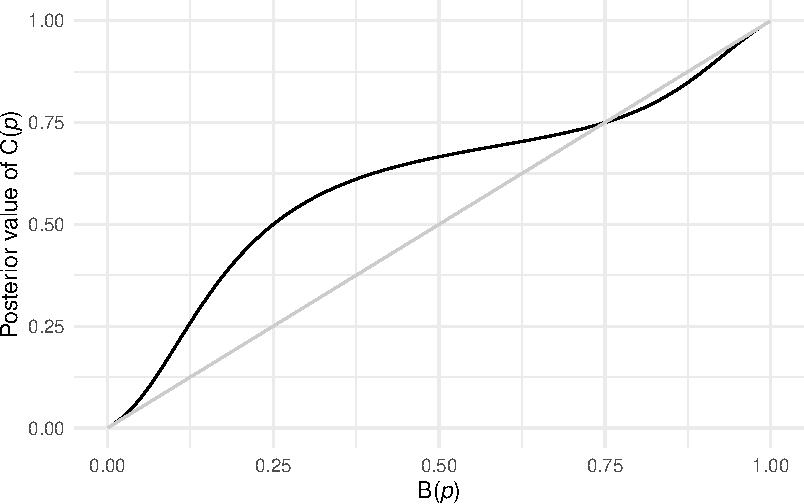
\includegraphics[keepaspectratio]{defer-infinite_files/figure-pdf/fig-two-experts-1.pdf}}

}

\caption{\label{fig-two-experts}The posterior probability of C(\emph{p})
given A(\emph{p})~=~0.75.}

\end{figure}%

The distribution loosely follows what Levinstein
(\citeproc{ref-Levinstein2015}{2015}) calls Thrasymachus's Principle.
The more opinionated of the two experts gets much stronger weight. You
can see this in part by seeing how close the above graph gets to
\emph{x}~=~\emph{y} at either extreme. But it's perhaps more vivid if we
plot the posterior probability that the coin landed Tails against the
different values of B(\emph{p}), as in
Figure~\ref{fig-two-experts-heads}.

\begin{figure}

\centering{

\pandocbounded{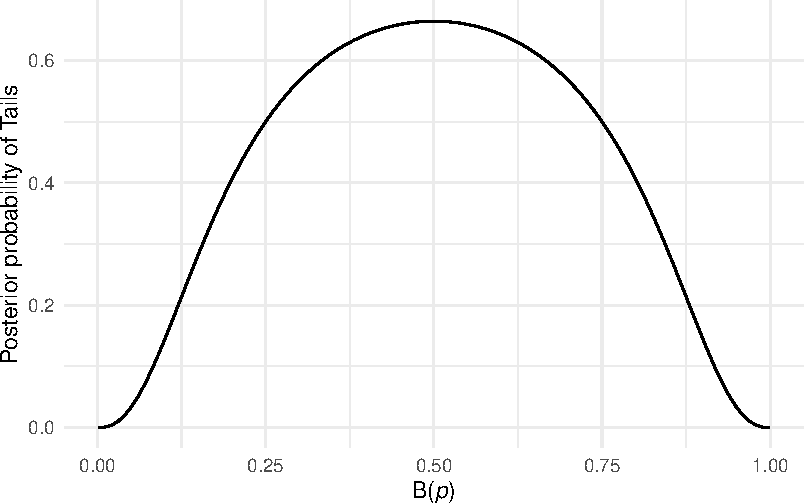
\includegraphics[keepaspectratio]{defer-infinite_files/figure-pdf/fig-two-experts-heads-1.pdf}}

}

\caption{\label{fig-two-experts-heads}The posterior probability of the
coin landing Tails given A(\emph{p})~=~0.75.}

\end{figure}%

When B(\emph{p}) is between 0.25 and 0.75, i.e., when it is closer to
0.5 than A(\emph{p}) is, C is confident that the coin landed Tails, and
that A is more informed and hence more worthy of deference. When
B(\emph{p}) takes a more extreme value, then C is confident that the
coin landed Heads, and hence that B is more worthy of deference. In
general, this model backs up Levinstein's intuition that more
opinionated sources are probably better informed, and hence more worthy
of deference.

\section{Evidence and Nesting}\label{sec-nesting}

The previous section assumed that C strongly deferred to A and B. We now
turn to the question of when C should do that. A natural thought, one we
relied on in that discussion, was that C should defer when they regard A
and B as better informed than they are. This can be motivated with a
famous result from David Blackwell (\citeproc{ref-Blackwell1953}{1953}).
Let E\textsubscript{1} and E\textsubscript{2} be functions from W to
subsets of W. Intuitively, these are \emph{experiments}; The
Experimenter will perform E\textsubscript{\emph{i}} and learn they are
in E\emph{\textsubscript{i}}(\emph{w}), where \emph{w} is the world they
are in. Blackwell assumes that the range of each
E\textsubscript{\emph{i}} is a partition of W; The Experimenter always
learns what cell of the partition they are in.

The short version of the big result is that E\textsubscript{1} is
guaranteed to be more valuable than E\textsubscript{2} iff
E\textsubscript{1} is more informative than E\textsubscript{2}. All of
that needs clarifying though.

Say E\textsubscript{1} is a \emph{refinement} of E\textsubscript{2} iff
for all \emph{w},
E\textsubscript{1}(\emph{w})~⊆~E\textsubscript{2}(\emph{w}). Formally,
this is how we'll capture the intuitive notion of being more
informative.\footnote{Note that comparisons here always include
  equality. An experiment is a refinement of itself, is more informative
  than itself, and is more valuable than itself. This can lead to
  confusion, but it's the standard terminology, and the alternative is
  much more wordy.}

Let O be a finite set of options:
\{O\textsubscript{1},~\ldots,~O\textsubscript{\emph{n}}\}. Each
O\textsubscript{\emph{i}} is a function from W to reals. Intuitively,
they are bets, and the number is the return on each bet. I'll follow
standard terminology in philosophy and say that a function from worlds
to reals is a \emph{random variable}. Given a random variable X (defined
on W) and a probability function Pr, we can define the expectation
Exp(W, Pr) as ΣPr(\emph{w})X(\emph{w}), where the sum is across members
of W.\footnote{I'm defining random variable and expected value the way
  they are usually defined in philosophy. In some fields it is more
  common to define random variables as functions from a probability
  space to reals, where a probability space has W and Pr as
  constituents. Then we can define expectation as a one-place function
  that simply takes a random variable as input. I think the
  philosophers' way of speaking is more useful, and in any case I'm a
  philosopher so it's more natural to me. But note there is a potential
  terminological confusion here.}

Say a strategy S is a function from E and W to O such that if
E(\emph{x})~=~E(\emph{y}), then S(\emph{x})~=~S(\emph{y}). That is,
strategies are not more fine-grained than evidence. Intuitively, a
strategy is something that The Experimenter can implement given their
evidence, so it can't require them to make more discriminations than
their evidence does. For each S, we can define a random variable
S\textsubscript{R} (read this as the return of S), such that
S\textsubscript{r}(\emph{w})~=~S(\emph{w})(\emph{w}). In words, the
return of S at \emph{w} is the value at \emph{w} of the option S selects
at \emph{w}.

Finally, say that a strategy is \textbf{recommended}\footnote{This term
  is taken from Dorst et al. (\citeproc{ref-DorstEtAl2021}{2021})} by Pr
(relative to E, O and W) just in case for all \emph{w} in W, and
alternative options O\textsubscript{a} in O,
Exp(S(\emph{w}),~Pr(•~\textbar~E(\emph{w})))~⩾~Exp(O\textsubscript{a},~Pr(•~\textbar~E(\emph{w}))).
In words, the option selected by S at \emph{w} has maximal expected
utility out of the options in O, relative to the result of updating Pr
on the evidence available at \emph{w}. Given these notions, we can state
two important results Blackwell proves.

First, for any O, W and Pr, if E\textsubscript{1} is a refinement of
E\textsubscript{2}, S\textsubscript{1} is recommended by
E\textsubscript{1} and S\textsubscript{2} is recommended by
E\textsubscript{2}, then Exp(S\textsubscript{1},
Pr)~⩾~Exp(S\textsubscript{2}, Pr). No matter what practical problem The
Experimenter is facing, and no matter what their priors are, they are
better off adopting a strategy recommended by the more informative
experiment.

Second, for any W, if E\textsubscript{1} is not a refinement of
E\textsubscript{2}, then for some O and Pr, there exists an
S\textsubscript{1} is recommended by E\textsubscript{1} and
S\textsubscript{2} is recommended by E\textsubscript{2} such that
Exp(S\textsubscript{1}, Pr)~\textless~Exp(S\textsubscript{2}, Pr). That
is, if E\textsubscript{1} is not more informative than
E\textsubscript{2}, then for some practical problem, it is better in
expectation to perform E\textsubscript{2} and carry out some strategy
recommended by it.

Blackwell isn't the first to connect the value of experiments to the
relative value of strategies and options in this way; for some history
of this idea see Das (\citeproc{ref-Das2023}{2023}) and Cam
(\citeproc{ref-LeCam1996}{1996}). But he works out the consequences of
it in much more detail than anyone had before him. (The two results I've
listed here don't go close to exhausting what he proved, but they are
enough for our purposes.) Philosophers have primarily focussed on the
first of these two results. And they have focussed largely on the
special case when E\textsubscript{2}(\emph{w})~=~W; i.e., when
`performing' experiment E\textsubscript{2} means getting no information
at all.\footnote{Further, they haven't always credited Blackwell (or the
  earlier results from Peirce and Ramsey that Das discusses) when they
  do discuss the results. We're grateful to John Quiggin for pointing
  out to us the importance of Blackwell's results in this context.} In
this section we'll also ignore the second result, but we will pay
attention to the case where E\textsubscript{2} isn't universal.

John Geanakoplos (\citeproc{ref-Geanakoplos1989}{{[}1989{]} 2021})
proved an interesting generalisation of this first result. As noted
earlier, Blackwell's theorems presuppose that each experiment is
partitional. Formally, E is partitional iff for all \emph{w},
\emph{w}~∈~E(\emph{w}), and for all \emph{w},~\emph{v}, if \emph{v} ∈
E(\emph{w}), then E(\emph{w})~=~E(\emph{v}). Geanakoplos shows something
interesting about experiments that are reflexive, transitive, and
nested. These are defined as follow (with leading quantifiers over
worlds left implicit)

\begin{description}
\tightlist
\item[Reflexive]
\emph{w} ∈ E(\emph{w}).
\item[Transitive]
If \emph{v} ∈ E(\emph{w}), then E(\emph{w}) ⊆ E(\emph{v}).
\item[Nested]
Either E(\emph{w})~∩ E(\emph{v}) = ∅, or E(\emph{w}) ⊆ E(\emph{v}), or
E(\emph{v}) ⊆ E(\emph{w}).
\end{description}

He shows that both the results of Blackwell's described above continue
to hold when E\textsubscript{1} is reflexive, transitive, and nested, as
long as E\textsubscript{2} is partitional.

This result has had some influence on recent philosophical work. It
suggests the following kind of argument.

\begin{enumerate}
\def\labelenumi{\arabic{enumi}.}
\tightlist
\item
  Performing experiments is valuable.
\item
  Performing experiments is valuable iff experiments are nested.
\item
  Therefore, experiments are nested.
\end{enumerate}

That's fairly crude as stated, but it's possible to develop it into a
more sophisticated argument that has implications for what the correct
epistemic logic should be. You can (more sophisticated) versions of this
argument in Spencer (\citeproc{ref-Spencer2018}{2018}) and Dorst
(\citeproc{ref-Dorst2019}{2019}), and criticisms of these arguments in
Williamson (\citeproc{ref-Williamson2019}{2019}) and Das
(\citeproc{ref-Das2023}{2023}).

The aim of this section is to show that two of the assumptions that
Geanakoplos uses in proving these results are essential. First,
E\textsubscript{2} has to be partitional; it is not sufficient that it
is reflexive, transitive, and nested. Second, it cannot be that both W
and O are infinite. Both results arguably help the Williamson-Das side
of the debate mentioned in the previous paragraph, but we won't go into
that in more detail here. The aim is just to show the formal limits of
Geanakoplos's result.

Here is the model that shows that more refined experiments do not
necessarily have higher expected value if both experiments are
reflexive, transitive, and nested.

\begin{itemize}
\tightlist
\item
  W = \{w\textsubscript{1}, w\textsubscript{2}, w\textsubscript{3}\}
\item
  Pr(w\textsubscript{1})~=~Pr(w\textsubscript{2})~=~Pr(w\textsubscript{3})~=
  ⅓
\item
  O = \{O\textsubscript{1}, O\textsubscript{2}\}
\item
  O\textsubscript{1}(w\textsubscript{1})~=
  O\textsubscript{1}(w\textsubscript{2})~=
  O\textsubscript{1}(w\textsubscript{3})~= 0
\item
  O\textsubscript{2}(w\textsubscript{1})~=~3
\item
  O\textsubscript{2}(w\textsubscript{2})~=~9
\item
  O\textsubscript{2}(w\textsubscript{3})~=~-6
\item
  E\textsubscript{1}(w\textsubscript{1})~=~\{w\textsubscript{1},~w\textsubscript{3}\}
\item
  E\textsubscript{1}(w\textsubscript{2})~=~\{w\textsubscript{2}\}
\item
  E\textsubscript{1}(w\textsubscript{3})~=~\{w\textsubscript{3}\}
\item
  E\textsubscript{2}(w\textsubscript{1})~=~\{w\textsubscript{1},~w\textsubscript{2},
  w\textsubscript{3}\}
\item
  E\textsubscript{2}(w\textsubscript{2})~=~\{w\textsubscript{2},
  w\textsubscript{3}\}
\item
  E\textsubscript{2}(w\textsubscript{3})~=~\{w\textsubscript{3}\}
\end{itemize}

Given no information, the optimal strategy is to always take the bet,
i.e., choose O\textsubscript{2} over the fixed return of 0 that is
O\textsubscript{1}. This has an expected return of 2. Given
E\textsubscript{1}, the only recommended strategy is to choose
O\textsubscript{1} at w\textsubscript{1} and w\textsubscript{3}, and
O\textsubscript{2} at w\textsubscript{2}, for an expected return of 2.
But given the less informative E\textsubscript{2}, the recommended
strategy is to choose O\textsubscript{2} at w\textsubscript{1} and
w\textsubscript{2}, and O\textsubscript{1} at w\textsubscript{3}, for an
expected return of 4. In this case, performing the less informative
experiment has higher expected returns. (Though to be clear, both
experiments have positive expected returns, relative to not doing
anything.)

Next we'll show the result does not hold when W and O are infinite. We
have to be careful here because it's easy to have a case where
S\textsubscript{1} and S\textsubscript{2} are undefined. And it's not
interesting that Exp(S\textsubscript{1},~Pr)~⩾~Exp(S\textsubscript{2},
Pr) might sometimes fail to be true simply because one or other term in
it isn't defined. So we'll restrict attention to cases where utilities
are bounded, for any E and any \emph{w} there is an optimal strategy
given E(\emph{w}), and the expectation of any recommended strategy is
defined.

Let W be the reals in (0,1).
E\textsubscript{1}(\emph{x})~=~{[}\emph{x},1), and
E\textsubscript{2}(\emph{x})~=~(0,1). For any \emph{x} in {[}0,1{]}, let
O\textsubscript{\emph{x}}(\emph{y}) be~-1 if \emph{x}~\geq~\emph{y}, and
\emph{x} if \emph{x}~\textgreater~\emph{y}, and O be the set of all
these O\textsubscript{\emph{x}}. And Pr is the flat distribution over
(0,1); the only fact we'll need is that whenever
0~\textless~\emph{x}~\textless~\emph{y}~\textless~1, the probability
that the actual world is in (\emph{x},~\emph{y}) is \emph{y}~-~\emph{x}.

The only strategy recommended by E\textsubscript{2} is to always choose
O\textsubscript{0}, which has a guaranteed return of 0. The strategy
recommended by E\textsubscript{1} is to choose O\textsubscript{\emph{x}}
upon learning that the true value is in (\emph{x},~1). That has an
expected return of \emph{x}, which is higher than all the alternatives.
But following that strategy all the time has a guaranteed return of -1,
which is worse than the strategy recommended by E\textsubscript{2}. And
that's true even though E\textsubscript{2} is partitional, and
E\textsubscript{1} is reflexive, transitive, and nested.

Now there is something odd about this example - each of the
O\textsubscript{\emph{x}} is discontinuous. In each case, the payouts
jump from -1 to \emph{x} at a particular point. This suggests a question
to which we don't know the answer: If every member of O is continuous,
are more refined experiments valuable in expectation? It is also unknown
whether Geanakoplos's results hold in countable frames. But what this
model shows is that if we allow discontinuous payouts, and uncountable
frames, the result does not hold.

\section{Trust and Value}\label{sec-dorst}

The role of experiments in the frames discussed in
Section~\ref{sec-nesting} is somewhat curious. They are in one respect
central, the theorems are all restricted to whether frames are
partitional, nested, etc, but they are in another respect ephemeral.
Ultimately what matters is not the experiment, but the probability that
The Experimenter has after performing an experiment. This latter way of
thinking is a helpful way to understand a striking recent result by
Dorst et al. (\citeproc{ref-DorstEtAl2021}{2021}).

Say a probability frame is an ordered pair ⟨W, P⟩ such that W is a set
(intuitively, of worlds), and P is a function from W to probability
functions defined on w. One way to generate such a pair is to have some
experiment E and prior probability Pr, each defined on W, and have
P(\emph{w}) be Pr(•~\textbar~E(\emph{w})). But you can just cut out the
E and Pr, and focus simply on W and P. As Dorst et al.
(\citeproc{ref-DorstEtAl2021}{2021}) show, this turns out to be
mathematically a very helpful move. It lets you see a lot more
interesting features of these frames.\footnote{At least in the case
  where W is finite; we'll be getting to the issues when it is not.}
They call frames where P is generated from E and Pr in this way
\emph{prior frames}, and those will be the focus of discussion here, but
it is interesting to see them as a special case of a more general class.

One thing they prove by looking at the more general class is that when W
is finite, the following two claims are equivalent. (I'll state the
claims formally, then explain my notation.)

\begin{description}
\tightlist
\item[Total Trust]
E(X~\textbar~\{\emph{w}:~Exp(X,~P(\emph{w}))~⩾~\emph{t}\},~π)~⩾~\emph{t}
\item[Value]
If O is a set of options, \emph{s} is a recommended strategy for O, and
\emph{o} is a member of O, then Exp(\emph{s},~π)~⩾~E(\emph{o},~π).
\end{description}

There is a bit there to unpack. We'll follow them in using π for a
probability function that is outside the frame. We'll sometimes call it
Novice's probability function, as opposed to P(\emph{w}) which is The
Experimenter's probability function at \emph{w}.\footnote{When the frame
  is a prior frame, it is natural to focus on the case where π~=~Pr, but
  again we're not just looking at prior frames.} We're generalising the
notion of expectation a bit to allow for conditional expectations;
Exp(X~\textbar~p,~Pr) is the expectation of X according to
Pr(•~\textbar~p). So here's what Total Trust says. Take any random
variable X. Update π on the proposition that consists of all and only
worlds where The Experimenter at that world has an expected value for X
at least equal to \emph{t}. After that update, Novice also expects X's
value to be at least \emph{t}.

We discussed recommended strategies in Section~\ref{sec-nesting}, so
there is less to say about Value. What it says is that Novice does not
expect any member of O to do better than any recommended strategy.

One way Dorst et al put the equivalence between Total Trust and Value
(on finite frames) is that π Totally Trusts a frame ⟨W, P⟩ iff it Values
that frame. What I'll show is that this equivalence breaks down when we
drop the finiteness assumptions. Indeed, it breaks down even when W is
countably infinite.

Start with a frame I'll call \textbf{Coin}. A fair coin will be flipped
repeatedly until it lands Tails. Let F be a random variable such that
F~=~\emph{x} iff the coin is flipped \emph{x} times. (If the coin never
lands Tails, we'll stipulate that F~=~1. Since this has probability 0,
it doesn't make a difference to the probabilities, but it will make a
difference to the possible choices post-update.) Novice knows these
facts about F, so π(F~=~\emph{x})~=~2\textsuperscript{-\emph{x}}. If
F~=~\emph{x}, then The Experimenter learns F~⩾~\emph{x} and nothing
else, and updates on that. That is,
P(F~=~\emph{x})~=~π(•\textbar F~⩾~x). For any positive integer \emph{i},
let O\textsubscript{i} be the random variable that takes value 0 at
F~=~\emph{j}~when \emph{j}~⩽~\emph{i}, and value
2\textsuperscript{\emph{i}} at F~=~\emph{j} when \emph{j}~\textgreater{}
\emph{i}. Let O be the set of each O\textsubscript{\emph{i}}. The
strategy \emph{s} such that
\emph{s}(F~=~\emph{i})~=~O\textsubscript{\emph{i}} is recommended, as
can be easily checked. But E(\emph{s})~=~0, while for any \emph{o} ∈~O,
E(\emph{o},~π)~= ½. So Value fails on \textbf{Coin}.

On the other hand, π does Totally Trust \textbf{Coin}. For any random
variable X and threshold \emph{t}, say an integer \emph{k} is a cut-off
if either Exp(X~\textbar~F~⩾~\emph{k},~π)~⩾~\emph{t} and
Exp(X~\textbar~F~⩾~\emph{k}~+~1,~π)~\textless~\emph{t}, or
Exp(X~\textbar~F~⩾~\emph{k},~π)~\textless~\emph{t} and
Exp(X~\textbar~F~⩾~\emph{k}~+~1,~π)~⩾~\emph{t}. Let
c\textsubscript{\emph{i}} be the \emph{i}'th cutoff. Partition the
integers into the regions between cutoffs. More precisely, do the
following. If 1 is not a cutoff, the first cell of the partition is
\{1,~\ldots,~c\textsubscript{1}-1\}; otherwise the first cell is just
\{1\}. If there is a last cutoff \emph{c}, the last cell is
\{c,~c+1,~\ldots\}. Otherwise, each cell is
\{c\textsubscript{\emph{i}},~\ldots,~c\textsubscript{\emph{i}+1}-1\}.
Say a cell is \emph{positive} if for every \emph{k} in it,
Exp(X~\textbar~F~⩾~\emph{k},~π)~⩾~\emph{t}, and negative otherwise. (By
the construction of the cells,
Exp(X~\textbar~F~⩾~\emph{k},~π)~⩾~\emph{t} is true for either all or
none of the members.)

Let \{c\textsubscript{\emph{i}},~\ldots,~c\textsubscript{\emph{i}+1}-1\}
be an arbitrary positive cell. By construction,
Exp(X~\textbar~F~⩾~c\textsubscript{\emph{i}},~π) ⩾~\emph{t}, and
Exp(X~\textbar~F~⩾~c\textsubscript{\emph{i}+1},~π)~\textless~\emph{t}.
Since for some λ ∈ (0,1),
Exp(X~\textbar~F~⩾~c\textsubscript{\emph{i}},~π) = λExp(X~\textbar~F~∈
\{c\textsubscript{\emph{i}},~\ldots,~c\textsubscript{\emph{i}+1}-1\},~π)~+
(1-λ)Exp(X~\textbar~F~⩾~c\textsubscript{\emph{i}+1},~π), it follows that
Exp(X~\textbar~F~∈~\{c\textsubscript{\emph{i}},~\ldots,~c\textsubscript{\emph{i}+1}-1\},~π)
⩾~\emph{t}. Since this was an arbitrary positive cell, it follows that
Exp(X~\textbar~F~∈~I,~π)~⩾~\emph{t} for any positive cell I. Since
Exp(X~\textbar~\{\emph{w}:~Exp(X,~P(\emph{w}))~⩾~\emph{t}\},~π) is a
weighted average of the values of Exp(X~\textbar~F~∈~I,~π) where I is
one or other of the positive cells, it follows that
E(X~\textbar~\{\emph{w}:~Exp(X,~P(\emph{w}))~⩾~\emph{t}\},~π)~⩾~\emph{t},
as required.

So π Totally Trusts \textbf{Coin}, but doesn't Value it. So the
equivalence between Total Trust and Value fails here. But you might very
reasonably object on two scores. First, the value function used to
generate the counterexample was unbounded, and we know that unbounded
value functions lead to all sorts of paradoxes. Second, I didn't just
make W infinite, I made O infinite as well, so this isn't a minimal
generalisation of the original claim. It turns out that if we put both
these constraints on, then the equivalence fails in the other direction:
It is possible to get a frame that π Values, but does not Totally Trust.

Call the following frame \textbf{Bentham}. Again, a coin will be flipped
until it lands Tails. If it ever lands Tails, F is the number of flips.
If it never lands Tails, which has probability 0, then F~=~∞. Again,
Novice knows these facts, and so far the case is just like
\textbf{Coin}. But in this case, if F~=~\emph{x}, The Experimenter
learns that F~⩽~\emph{x} and nothing else, and The Experimenter updates
on that. So if F~=~∞, The Experimenter learns nothing, but otherwise
they can rule out all but finitely many possibilities. More precisely,
P(F~=~\emph{x})~=~π(•\textbar F~⩽~x).

The Novice probability does not Totally Trust this frame. Let Y be a
random variable such that Y(F~=~∞) = 0, and for all finite \emph{n},
Y(F~=~\emph{n}) = 1 - 2\textsuperscript{-\emph{n}}.
E(Y~\textbar~\{\emph{w}:~Exp(Y,~P(\emph{w}))~⩾~⅔\},~π) =~0~\textless{}
⅔. The only world \emph{w} where Exp(Y,~P(\emph{w}))~⩾~⅔ is F~=~∞, and
at F~=~∞, Y~=~0.

On the other hand, π does Value this frame. To see this, for any set of
options O, recommended strategy S, random variable X (all defined on W),
and integer \emph{n}, let W\emph{n} be the set \{F~=~1, \ldots,
F~=~\emph{n}\}, O\textsubscript{\emph{n}}, P\textsubscript{\emph{n}},
S\textsubscript{\emph{n}} and X\textsubscript{\emph{n}} be the
restrictions of O, P and S to worlds in W\emph{n}. From the way P is
constructed, i.e., by conditionalising on the set of worlds where F is
no greater than it actually is, it follows that if S is recommended on
⟨W,~P⟩, then S\textsubscript{\emph{n}} is recommended on
⟨W\textsubscript{\emph{n}},~P\textsubscript{\emph{n}}⟩. Since
⟨W\textsubscript{\emph{n}},~P\textsubscript{\emph{n}}⟩ is a finite prior
frame where E is reflexive, transitive and nested, and Pr~=~π, it
follows by the result of Geanakoplos described in
Section~\ref{sec-nesting}, that the expected return of
S\textsubscript{\emph{n}} is greater than the expected return of any
option in O\textsubscript{\emph{n}}. For any random variable X,
Exp(X,~π) is the limit as \emph{n} tends to ∞ of
Exp(X\textsubscript{\emph{n}},~π); this is because as \emph{n} grows
this covers all words in W except F~=~∞, which has probability 0. If the
expected return of S is the limit \emph{n} tends to ∞ of the expected
return of S\emph{\textsubscript{n}}, and the expected return of an
option in O is the limit as \emph{n} tends to ∞ of its counterpart in
O\textsubscript{\emph{n}}, and S\emph{\textsubscript{n}} is better (in
expectation) than every option in O\textsubscript{\emph{n}}, it follows
that S is better (in expectation) than every option in O. So Value is
satisfied, as required.

\section{Conclusion}\label{conclusion}

It's striking that we get such different behaviours between finite and
infinite frames when it comes to these three somewhat distinct issues
about deference and updating. The main point of this note is to point
out these differences.

But there is a broader philosophical question. One might think that
since humans are finite, results that hold on all finite frames should
be used when thinking about humans. I think this is a bit quick. All the
models we've been using here, both the finite and the infinite ones,
really are \emph{models}. Even the finite ones assume that the people
being modeled have superhuman (if not literally infinite) computational
capacities. They are all idealisations. The question is, are they good
or bad idealisations? Here the issues about finitude get complicated. It
might be that an infinite model is a better idealisation, a better
approximation to a human than a finite one.

Imagine someone saying that since humans are finite, and circles are
infinitely curved, we should never model humans as thinking about
circles. Rather, we should think that the human is thinking of a regular
polygon with arbitrarily many sides. This is a little absurd. A model
where the human is thinking of a circle is simpler than a model where
the human is thinking, in full precision, about a chiliagon. By the same
reasoning, it might be better to model a scientist as taking some
variable to be normally distributed over an interval, than to take them
to have in their head a particular finite approximation to the normal
distribution, which they perfectly update. For that reason, the model in
Section~\ref{sec-gallow} might be a decent model of deference.

The models in Section~\ref{sec-nesting} are, admittedly, weirder. There
is less use, even in idealisations, for infinite models with
discontinuous payouts, or for models with unbounded utility functions.
These are known to lead to weird results. Here I think there is a
stronger claim that the models I've presented are not useful models, not
because they are infinite, but because they are discontinuous and
unbounded.

But there is obviously much more to say about these questions about
usefulness. Hopefully it is helpful to simply point out how differently
the finite and infinite cases behave.

\subsection*{References}\label{references}
\addcontentsline{toc}{subsection}{References}

\phantomsection\label{refs}
\begin{CSLReferences}{1}{0}
\bibitem[\citeproctext]{ref-Blackwell1951}
Blackwell, David. 1951. {``Comparison of Experiments.''}
\emph{Proceedings of the Berkeley Symposium on Mathematical Statistics
and Probability} 2 (1): 93--102.

\bibitem[\citeproctext]{ref-Blackwell1953}
---------. 1953. {``Equivalent Comparisons of Experiments.''} \emph{The
Annals of Mathematical Statistics} 24 (2): 265--72.

\bibitem[\citeproctext]{ref-LeCam1996}
Cam, L. Le. 1996. {``Comparison of Experiments: A Short Review.''} In
\emph{Statistics, Probability and Game Theory: Papers in Honor of David
Blackwell}, edited by T. S. Ferguson, L. S. Shapley, and J. B. MacQueen,
127--38. Hayward, CA: Institute of Mathematical Statistics. doi:
\href{https://doi.org/10.1214/lnms/1215453569}{10.1214/lnms/1215453569}.

\bibitem[\citeproctext]{ref-Das2023}
Das, Nilanjan. 2023. {``The Value of Biased Information.''}
\emph{British Journal for the Philosophy of Science} 74 (1): 25--55.
doi: \href{https://doi.org/10.1093/bjps/axaa003}{10.1093/bjps/axaa003}.

\bibitem[\citeproctext]{ref-Dorst2019}
Dorst, Kevin. 2019. {``Evidence: A Guide for the Uncertain.''}
\emph{Philosophy and Phenomenological Research} 100 (3): 586--632. doi:
\href{https://doi.org/10.1111/phpr.12561}{10.1111/phpr.12561}.

\bibitem[\citeproctext]{ref-DorstEtAl2021}
Dorst, Kevin, Benjamin A. Levinstein, Bernhard Salow, Brooke E. Husic,
and Branden Fitelson. 2021. {``Deference Done Better.''}
\emph{Philosophical Perspectives} 35 (1): 99--150. doi:
\href{https://doi.org/10.1111/phpe.12156}{10.1111/phpe.12156}.

\bibitem[\citeproctext]{ref-Gallow2018}
Gallow, J. Dmitri. 2018. {``No One Can Serve Two Epistemic Masters.''}
\emph{Philosophical Studies} 175 (10): 2389--98. doi:
\href{https://doi.org/10.1007/s11098-017-0964-8}{10.1007/s11098-017-0964-8}.

\bibitem[\citeproctext]{ref-Geanakoplos1989}
Geanakoplos, John. (1989) 2021. {``Game Theory Without Partitions, and
Applications to Speculation and Consensus.''} \emph{The B.E. Journal of
Theoretical Economics} 21 (2): 361--94. doi:
\url{https://doi.org/10.1515/bejte-2019-0010}.

\bibitem[\citeproctext]{ref-Levinstein2015}
Levinstein, Benjamin Anders. 2015. {``With All Due Respect: The
Macro-Epistemology of Disagreement.''} \emph{Philosophers' Imprint} 15
(13): 1--20.

\bibitem[\citeproctext]{ref-Spencer2018}
Spencer, Jack. 2018. {``No Crystal Balls.''} \emph{Noûs} 54 (1):
105--25. doi:
\href{https://doi.org/10.1111/nous.12252}{10.1111/nous.12252}.

\bibitem[\citeproctext]{ref-Williamson2019}
Williamson, Timothy. 2019. {``Evidence of Evidence in Epistemic
Logic.''} In \emph{Higher-Order Evidence: New Essays}, edited by Mattias
Skipper and Asbjørn Steglich-Petersen, 265--97. Oxford: {O}xford
{U}niversity {P}ress. doi:
\href{https://doi.org/10.1093/oso/9780198829775.003.0013}{10.1093/oso/9780198829775.003.0013}.

\end{CSLReferences}



\noindent \vspace{1in} In progress


\end{document}
